
\exo

On donne le graphique suivant où il a été représentée la courbe représentative de la fonction $f$.

\begin{center}
\psset{xunit=0.7cm,yunit=0.7cm,algebraic=true}
\begin{pspicture*}(-5.2,-4.3)(7,3)
\small
\psgrid[gridlabels=0,griddots=10,subgriddiv=0](-5,-4)(7,4)
\psaxes{->}(0,0)(-5,-4)(7,3)
\pscurve{-}(-5,-1)(-1,-2)(1.5,2)(4,0)(6,-3)
\end{pspicture*}
\end{center}
%\vspace*{0.5cm}
\begin{enumerate}
\item Par lecture graphique, compléter le tableau de valeurs suivants :

\begin{tabularx}{0.7\linewidth}{|*{8}{>{\centering\arraybackslash}X|}}
\hline 
$x$&-5&-3&-1&0&2&4&6 \\
\hline
$f(x)$& & & & & & & \\
\hline
\end{tabularx}

\item Dresser le tableau de variations de $f$.
\item Dresser le tableau de signes de $f$.
\end{enumerate}

\medskip

\exo 

A l'aide de votre calculatrice, compléter le tableau de valeurs suivant pour la fonction $g$ définie par $g(x)= x^3 -5x^2 + 3x + 5$ :

\medskip

\begin{tabularx}{0.99\linewidth}{|*{10}{>{\centering\arraybackslash}X|}}
\hline 
$x$&-2&-1&0&1&2&3&4&5&6 \\
\hline
$g(x)$& & & & & & & & &\\  
\hline
\end{tabularx}

\medskip

Représenter graphiquement la fonction sur votre calculatrice en choisissant une fenêtre adaptée.


\medskip

Compléter votre choix :

\begin{center}
\begin{tabular}{|lc|}
\hline
Xmin = &~~~~~~\\
Xmax = &\\
scale =& 1\\
Ymin = &\\
Ymax = &\\
scale =& 1\\
\hline
\end{tabular}
\end{center}

\medskip

\exo 

\begin{enumerate}
\item Représenter sur votre cahier d'exercice la fonction $f$ définie par $f(x)= 2x^2 - 6x + 2$. On construira d'abord un tableau de valeurs de -0,5 à 4,5 avec un pas de 0,5.
\item Dresser le tableau de variation de $f$.
\item Pourquoi peut-on affirmer que $f$ admet un minimum ? 

Quel est ce minimum ?
\item Représenter sur le \textbf{même} graphique la représentation de la fonction $g$ définie par $g(x)= 2-x$
\item Résoudre graphiquement $f(x)> g(x)$.
\end{enumerate}


\exo

Soit $f$ la fonction définie sur $\R$ par $f(x)= x^2-8x+3$

\begin{enumerate}
\item Montrer que $f(x)=(x-4)^2 - 13$
\item Justifier que pour tout $x$ réel, $f(x) \geqslant -13$
\item En déduire que $f$ admet un minimum et donner ce minimum. 
\item Pour quelle valeur est-il atteint ?
\item Tracer la courbe sur votre calculatrice pour vérifier.
\end{enumerate}

\medskip

\exo

Soit $g$ la fonction définie sur $\R$ par $g(x)= -x^2 +6x -5$
\begin{enumerate}
\item Montrer que $f(x)= -(x-3)^2 + 4$
\item Justifier que $f$ admet un maximum sur $\R$
\end{enumerate}

\medskip

\exo

\textbf{partie A :}

\medskip

\begin{enumerate}
\item Tracer la courbe représentative de la fonction $f$ définie sur $[ -1 ; 4 ]$ par $f(x) = x^2-2x$
\item Résoudre graphiquement $f(x) = 5$ puis $f(x) = -2$ 

\item Quels sont les antécédents de 0 par $f$ ?

\item Résoudre graphiquement $f(x) = 0$ puis $f(x)\geq 0$

\item Justifier que $f$ admet un minimum pour $x=1$
\item Montrer que $f(a)-f(b)=(a-b)(a+b-2)$
\item Etudier les variations de $f$ sur $[1 ;+\infty[$ puis dresser le tableau de variation de $f$ sur $\R$. 
\end{enumerate}

\medskip

\textbf{partie B :}

\medskip

\begin{enumerate}
\item Tracer sur le graphique la droite représentant la fonction $g$ définie par $g(x) = x-2$
\item Résoudre $f(x) = g(x)$ puis $f(x)\leq g(x)$ graphiquement.
\end{enumerate}

\medskip

\exo 


\begin{enumerate}
\item Tracer la courbe représentative de la fonction $f$ définie par $f(x) = - x^2 + 4 x - 3$
\item Factoriser $f(a)-f(b)$ par $(a-b)$
\item Etudier les variations de $f$ sur  $]-\infty ; 2]$ 
\item Démontrer que $f$ admet un maximum en 2.
\item Vérifier que $f(x) = (x-3)(1-x)$ puis résoudre $f(x)=0$.
\end{enumerate}

\exo

\begin{minipage}{0.5\linewidth}
\psset{unit=1cm,algebraic =true}
\begin{pspicture*}(-4.2,-4.2)(4.5,4.5)
\psplot[linecolor=blue,linewidth=1.3pt]{-4}{4}{1.5*x-2}
\psplot[linecolor=black,linewidth=1.3pt]{-4}{4}{-x+2}
\psplot[linecolor=orange,linewidth=1.3pt]{-4}{4}{-0.5*x+1}
\psplot[linecolor=red,linewidth=1.3pt]{-4}{4}{3*x}
\rput(-1.5,-3.5){$(d_1)$}
\rput(-2,1.5){$(d_2)$}
\rput(-1,2.7){$(d_3)$}
\rput(3,2){$(d_4)$}
\psaxes{->}(0,0)(-4.5,-4.5)(4.5,4.5)
\psgrid[subgriddiv=0,griddots=10,gridlabels=0](0,0)(-4,-4)(4,4)
\end{pspicture*}
\end{minipage}
\begin{minipage}{0.45\linewidth}

Déterminer par lecture graphique les équations (réduites) des quatre droites tracées dans le repère ci-contre :

\vspace{0.5cm}

$(d_1) : $ \dotfill

\vspace{0.5cm}

$(d_2) : $ \dotfill

\vspace{0.5cm}

$(d_3) : $ \dotfill

\vspace{0.5cm}

$(d_4) : $ \dotfill


\vspace{2cm}

~
\end{minipage}



\exo

\begin{minipage}[t]{0.5\linewidth}
Dans le repère ci-contre :

Tracer les droites données par les équations suivantes :

a) $(d_1) : y = 3x -4$

c) $(d_2) : y =5-2x$

\end{minipage}
\begin{minipage}[t]{0.5\linewidth}
\psset{unit=0.9cm,algebraic =true}
\begin{pspicture*}(-5.2,-5.2)(5.5,5.5)
\psaxes{->}(0,0)(-5.5,-5.5)(5.5,5.5)
\psgrid[subgriddiv=0,griddots=10,gridlabels=0](0,0)(-5,-5)(5,5)
\end{pspicture*}

\end{minipage}

\exo

On considère la droite $(d)$ d'équation $ y = 5x - 7$

a) Sans tracer la droite, le point $B( -2 ; 1)$ appartient-il à la droite $(d)$  ? (justifier en écrivant un calcul)


b) même question avec le point $C(2 ;3)$



\exo

On considère les points $A(2 ; 11)$ et $B(-3 ; 1)$ 

Déterminer par le calcul l'équation réduite de la droite $(AB)$

\exo 

Pour chaque équation de droite ci-dessous, donner le coefficient directeur et l'ordonnée à l'origine :

\medskip


a) $y= 2x + 5$ 

\medskip

b) $y=-3x$

\medskip

c) $ y = \dfrac{2x+5}{8}$

\medskip

d) $y = 3 - 0,5x$ 

\medskip

\exo 

Dans le repère ci-dessous on a tracé les droites et  $(d_1)$, $(d_2)$, $(d_3)$ et $(d_4)$ représentants quatre fonctions affines $f_1$, $f_2$, $f_3$ et $f_4$, déterminer par lecture l'expression de chacune de ces fonctions.

\begin{center}
\psset{algebraic=true,unit=0.7}
\begin{pspicture*}(-4.1,-4)(5,5)
\psgrid[gridlabels=0,griddots=10,subgriddiv=2,subgriddots=5](0,0)(-4,-4)(5,5)
\psaxes[labelFontSize=\scriptstyle]{->}(0,0)(-5,-5)(5,5)
\psplot{-4}{5}{0.5*x-2}
\psplot{-4}{5}{-2*x+1}
\psplot{-5}{5}{2-0.66667*x}
\psplot{-5}{5}{3}
\rput(-1.2,4.3){$(d_4)$}
\rput(-3.5,-3){$(d_3)$}
\rput(4.5,-1.6){$(d_2)$}
\rput(-3,2.5){$(d_1)$}
\end{pspicture*}
\end{center}

\medskip

\exo 

Déterminer les équations des droites tracées ci-dessous :

\begin{center}
\psset{algebraic=true,unit=0.7}
\begin{pspicture*}(-4.1,-4)(5,5)
\psgrid[gridlabels=0,griddots=10,subgriddiv=2,subgriddots=5](0,0)(-4,-4)(5,5)
\psaxes[labelFontSize=\scriptstyle]{->}(0,0)(-5,-5)(5,5)
\psplot{-4}{5}{-0.25*x+3}
\psplot{-4}{5}{-2*x-1}
\psplot{-5}{5}{0.5*x}
\psplot{-5}{5}{x+2}
\rput(-2.2,4.3){$(d_4)$}
\rput(-1.5,-1.5){$(d_3)$}
\rput(2,-3.6){$(d_2)$}
\rput(-3.5,3.2){$(d_1)$}
\end{pspicture*}
\end{center}

\medskip

\exo 

On donne $A( 3 ; 4)$ ,  $B(2 ; 3,5)$ et $C(6; 5,5)$

\begin{enumerate}
\item Déterminer l'équation de la droite $(AB)$
\item Les points $A$ , $B$ et $C$ sont-ils alignés ?
\end{enumerate}


\exo 

La fonction $f$ est représentée par la droite $(AB)$ avec $A(-1 ;6)$ et $B(2; -6)$
\begin{enumerate}
\item Déterminer $f(x)$
\item Le point $C (\frac{1}{3} ; \frac{2}{3})$ appartient-il à la représentation graphique de $f$ ?
\end{enumerate}

\medskip

\exo

Déterminer la fonction affine $f$ permettant de convertir des degrés Celsius en degrés Fahrenheit sachant que 38 degrés Celsius correspond environ à 100 degrés Fahrenheit et qu'une température de 100 degrés Celsius correspond à 212 degrés Fahrenheit. (on arrondira les coefficients aux dixièmes)

\medskip

\exo

Indiquer si les fonctions affines suivantes sont croissantes ou décroissantes sur $\R$ :

\medskip

a) $f(x)= 3x + 5$

\medskip

b) $g(x)= -2x$

\medskip

c) $h(x)= 4-3x$

\medskip

d) $k(x)= \dfrac{-2x+7}{-3}$

\medskip

\exo 

Déterminer les équations des droites tracées ci-dessous :

\begin{center}
\psset{algebraic=true,unit=0.7}
\begin{pspicture*}(-4.1,-3.5)(5,5)
\psgrid[gridlabels=0,griddots=10,subgriddiv=2,subgriddots=5](0,0)(-4,-4)(5,5)
\psaxes[labelFontSize=\scriptstyle]{->}(0,0)(-5,-5)(5,5)
\psplot{-4}{5}{2-x}
\psplot{-4}{5}{1.5 -4*x}
\psplot{-5}{5}{0.66667*x}
\psplot{-5}{5}{1.5*x-2}
\rput(-1.5,4.6){$(d_4)$}
\rput(-1.5,-1.5){$(d_3)$}
\rput(3.5,4.2){$(d_2)$}
\rput(-2.5,3.7){$(d_1)$}
\end{pspicture*}
\end{center}

\exo 

Compléter le tableau de signe de la fonction $f$ définie sur $\R$ par $f(x)= 2x - 6$

\medskip

\begin{center}
\begin{tikzpicture}
\tkzTabInit[lgt=4,espcl=2]%
{$x$/1,signe de $f(x)$/1}%
{$-\infty$,$\ldots$,$+\infty$}%
\tkzTabLine{ ,  , z ,  , }
\end{tikzpicture}
\end{center}

\exo

Dresser les tableaux de signes des fonctions affines suivantes sur $\R$

\begin{multicols}{2}
\begin{enumerate}
\item $f(x) = x-5$
\item $g(x)= -3x -15$
\item $h(x)= -5x +1$
\item $k(x)= 5x$
\item $i(x)= -7x +6$
\item $j(x)= \dfrac{5x -4}{3}$
\end{enumerate}
\end{multicols}

\medskip

\exo

Dresser le tableau de signes de 

\begin{multicols}{2}
\begin{enumerate}
\item $2x+3)(-x+1)$
\item $(5-2x)(3x+1)$
\end{enumerate}
\end{multicols}

\medskip

\exo 

\begin{multicols}{2}
\begin{enumerate}
\item Dresser le tableau de signes de $(-5x+1)(2x+1)$
\item En déduire les solutions de $(-5x+1)(2x+1)>0$
\end{enumerate}
\end{multicols}

\medskip

\exo

Résoudre (en utilisant un tableau de signes):

\begin{multicols}{2}
\begin{enumerate}
\item $(x+3)(1-2x) < 0$
\item $(2x+1)(3-x)\leqslant 0$
\item $(2x+5)(4x-3)\geqslant 0$
\item $ 2(2 - x)( 1 -2x) > 0$
\end{enumerate}
\end{multicols}

\medskip

\exo  

même consigne :

\begin{multicols}{2}
\begin{enumerate}
\item $-3x^2+4x >0$
\item $x^2-16 < 0$
\item $(x+5)(4 -5x) -(x+5)(x + 1) \geqslant 0$
\item $x^2 + 3x < x$
\item $(x-1)(2x+3)  \geqslant (x-1)^2$
\end{enumerate}
\end{multicols}

\medskip

\exo 

Dresser le tableau de signes de $\dfrac{7x +1}{x+2}$

\medskip

\exo

Résoudre dans $\R$ :

\begin{multicols}{2}
\begin{enumerate}
\item $\dfrac{3 -5x}{x-12}< 0$
\item $\dfrac{25x-1}{x+1}\geqslant 0$
\item $\dfrac{1-6x}{x^2 + 4} < 0$
\item $\dfrac{3}{(x-1)(x-6)} \geqslant 0$
\item $\dfrac{4x -1}{2x +3} > 3$
\item $ \dfrac{2x}{6x+1}< 2$
\end{enumerate}
\end{multicols}

